\documentclass[11pt, oneside]{article} 
\usepackage{geometry}
\geometry{letterpaper} 
\usepackage{graphicx}
	
\usepackage{amssymb}
\usepackage{amsmath}
\usepackage{parskip}
\usepackage{color}
\usepackage{hyperref}

\graphicspath{{/Users/telliott/Github/calculus_book/png/}}
% \begin{center} 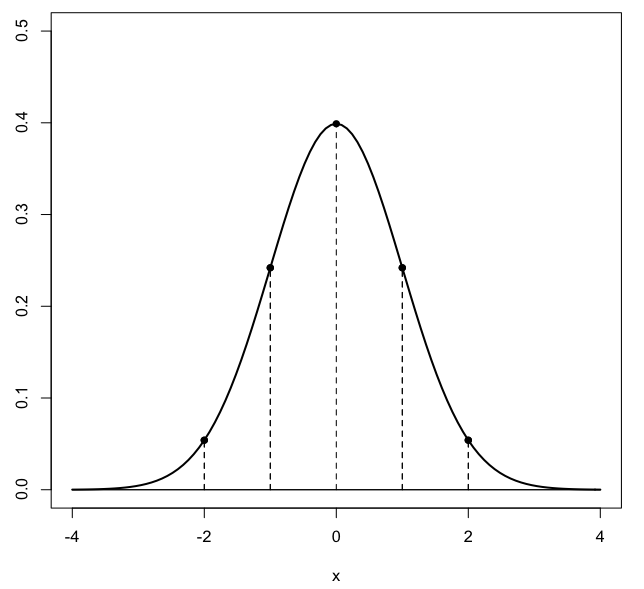
\includegraphics [scale=0.4] {gauss3.png} \end{center}

\title{Fundamental theorem of arithmetic}
\date{}

\begin{document}
\maketitle
\Large

This chapter doesn't have much to do with calculus, it is here because it is a key result of Euclid's, though he never stated the theorem in its modern form.  It also shows some more sophisticated but (I hope) not too challenging proofs.  It can be skipped without interfering with the development of the rest of the text.

We're going to show that every integer has a \textbf{unique prime factorization}.

\[ n = p_1 \cdot p_2 \dots p_n \]

First, we need a preliminary result, which is called \textbf{Euclid's lemma}.

Every natural number $n > 1$, i.e. every positive integer greater than $1$, is either prime, or it is the product of two smaller natural numbers $a$ and $b$.

But the same is true of $a$ and $b$ in turn.

Therefore, every number that can be factored into $a$ and $b$ is the product of the prime factors of $a$ times the prime factors of $b$.  

Suppose a given prime $p$ divides $n = ab$, i.e. $p|n$. Then either $p|a$ or  $p|b$ (or both).

\subsection*{Proof of existence}

The proof is by induction.  (I know we haven't covered induction yet, so you can consider this a demonstration of how the method works rather than a real proof.   For more information, see \hyperref[sec:induction]{\textbf{here}}.

Assume the lemma is true for all numbers between $1$ and $n$.  

It is certainly true for say, $n < 101$, because we can check each case.  Start with $n = 101$.

$\circ$ \ If $n$ is prime (as it is here) there is nothing to prove and we move to $n + 1$.  

$\circ$ \  $n$ is not prime, then there exist integers $a$ and $b$ (with $1 < a \le b < n$) such that $n = a \times b$.

$\circ$ \ By the induction hypothesis, since $a < n$ and $b < n$, $a$ has prime factors $p_1 p_2 \dots$ and $b$ has prime factors $q_1 q_2 \dots$ so
\[ n = ab = p_1 p_2 \dots q_1 q_2 \dots \]

This shows that there exists a prime factorization of $n$.

\subsection*{Proof of uniqueness}

To show that the prime factorization is unique suppose that $n$ is the smallest integer for which there exist two different factorizations:
\[ n = p_1 p_2 \dots = q_1 q_2 \dots \]
    
Pick the first factor $p_1$.  Since $p_1$ divides $n = q_1 q_2 \dots$, by Euclid's lemma, it must divide some particular $q_j$.  Rearrange the $q$ so that $q_j$ is first.

But since $p_1$ divides $q_1$ and both are prime, it follows that $p_1 = q_1$. 

Now continue the same process with all the factors $p_i$.

As wikipedia says now:

    This can be done for each of the $m$ $p_i$'s, showing that $m \le n$ and every $p_i$ is some $q_j$. Applying the same argument with the p and q reversed shows $n \le m$ (hence $m = n$) and every $q_j$ is a $p_i$.
    
\subsection*{Hardy proof}

Hardy and Wright (\emph{Theory of Numbers}, sect. 2:11) have a second proof, which is given here (almost) verbatim:

    Let us call numbers which can be factored into primes in more than one way, \emph{abnormal}, and let $n$ be the smallest abnormal number.

Different factorization:

The same prime $P$ cannot appear in two different factorizations of $n$, for, if it did, $n/P$ would be abnormal and yet $n/P < n$, the smallest abnormal number.

Thus, we have that

\[  = p_1 p_2 \dots = q_1 q_2 \dots \]
    
where the $p$ and $q$ are primes, and no $p$ is a $q$ and no $q$ is a $p$.

If there exist abnormal numbers with two such factorizations, they must be completely different.

\subsection*{the contradiction}

We may take $p_1$ to be the least $p$.  Since $n$ is composite, $p_1^2 \le n$.

The same is true for $q_1$ and (since $p_1 \ne q_1$), we have that $p_1 q_1 < n$

Hence, if $N = n - p_1 q_1$, we have $0 < N < n$ and also that $N$ is not abnormal.

Now $p_1 | n$ and since $N = n - p_1 q_1$, so $p_1 | N$.

Similarly $q_1 | N$.  Hence $p_1$ and $q_1$ both appear in the unique factorizations of both $N$ and $p_1 q_1$.

From this it follows that $p_1 q_1 | n$ and hence $q_1 = n/p_1$.  But $n/p_1$ is less than $n$ and has the unique prime factorization $p_2 p_3 \dots$.

Since $q_1$ is not a $p$, this is impossible.  Hence there cannot be any abnormal numbers, and this is the fundamental theorem.



\end{document}